\documentclass[a4paper,12pt]{article}
\usepackage{vntex}
\usepackage{mathptmx}[ptm]
\usepackage{a4wide,amssymb,epsfig,latexsym,array,hhline,fancyhdr}
\usepackage[normalem]{ulem}

\usepackage[makeroom]{cancel}
\usepackage{amsmath}
\usepackage{amsthm}
\usepackage{multicol,longtable,amscd}
\usepackage{diagbox}
\usepackage{booktabs}
\usepackage{alltt}
\usepackage[framemethod=tikz]{mdframed}
\usepackage{caption,subcaption}

\usepackage{lastpage}
\usepackage{enumerate}
\usepackage{color}
\usepackage{graphicx}
\let\oldincludegraphics\includegraphics
\renewcommand{\includegraphics}[2][]{%
  \oldincludegraphics[width=\textwidth,keepaspectratio,#1]{#2}%
}
\usepackage{pdfpages}
\usepackage{float}
\usepackage{array}
\usepackage{tabularx, caption}
\usepackage{multirow}
\usepackage{multicol}
\usepackage{rotating}
\usepackage{geometry}
\usepackage{setspace}
\usepackage{epsfig}
\usepackage{tikz}
\usepackage{url}

\renewcommand{\arraystretch}{1.3}

\usetikzlibrary{arrows,snakes,backgrounds,calc}
\usepackage[unicode]{hyperref}
\hypersetup{urlcolor=blue,linkcolor=black,citecolor=black,colorlinks=true}
\usepackage{listings}

\IfFileExists{grffile.sty}{\usepackage{grffile}}{}

\graphicspath{{../static/images/}{Images/}}

\def\thesislayout{
	\geometry{
		a4paper,
		total={160mm,240mm},
		left=30mm,
		top=30mm,
	}
}
\thesislayout

\lstset{
basicstyle=\footnotesize\ttfamily,
breaklines=true,
breakatwhitespace=false,
frame=single,
numbers=left,
numberstyle=\tiny,
stepnumber=1,
numbersep=5pt,
tabsize=2,
showspaces=false,
showstringspaces=false,
backgroundcolor=\color{white},
captionpos=b,
}

\setlength{\headheight}{40pt}
\pagestyle{fancy}
\fancyhead{}
\fancyhead[L]{
 \begin{tabular}{rl}
    \begin{picture}(25,15)(0,0)
    \put(0,-8){
\includegraphics[width=10mm, height=10mm]{Images/hcmut.png}}
   \end{picture}&
	\begin{tabular}{l}
		\textbf{  Trường Đại Học Bách Khoa - ĐHQG TP.HCM}\\
		\textbf{  Khoa Khoa Học \& Kỹ Thuật Máy Tính}
	\end{tabular}
 \end{tabular}
}
\fancyhead[R]{
	\begin{tabular}{l}
		\tiny \bf \\
		\tiny \bf
	\end{tabular}}
\fancyfoot{}
\fancyfoot[L]{\scriptsize  Báo cáo Thực tập Ngoài trường}
\fancyfoot[R]{\scriptsize  Trang {\thepage}/\pageref{LastPage}}
\renewcommand{\headrulewidth}{0.3pt}
\renewcommand{\footrulewidth}{0.3pt}

\setcounter{secnumdepth}{4}
\setcounter{tocdepth}{3}
\makeatletter
\newcounter{subsubsubsection}[subsubsection]
\renewcommand\thesubsubsubsection{\thesubsubsection .\@alph\c@subsubsubsection}
\newcommand\subsubsubsection{\@startsection{subsubsubsection}{4}{\z@}%
                                     {-3.25ex\@plus -1ex \@minus -.2ex}%
                                     {1.5ex \@plus .2ex}%
                                     {\normalfont\normalsize\bfseries}}
\newcommand*\l@subsubsubsection{\@dottedtocline{3}{10.0em}{4.1em}}
\newcommand*{\subsubsubsectionmark}[1]{}
\makeatother

\everymath{\color{black}}
\sloppy
\captionsetup[figure]{labelfont={small,bf},textfont={small,it},belowskip=-1pt,aboveskip=-9pt}
\captionsetup[table]{labelfont={small,bf},textfont={small,it},belowskip=-1pt,aboveskip=7pt}
\setlength{\floatsep}{5pt plus 2pt minus 2pt}
\setlength{\textfloatsep}{5pt plus 2pt minus 2pt}
\setlength{\intextsep}{10pt plus 2pt minus 2pt}

\thesislayout

% Cover-page text sizes, held to the official template's required 15pt/18pt
% exactly. The titlepage used to overflow onto a second page; fixed via
% \coverlistspacing (tighter itemize spacing) and \enlargethispage/\vfill
% below rather than by shrinking these sizes below what's required.
\newcommand{\cover}{\fontsize{15}{18}\selectfont}
\newcommand{\coverbig}{\fontsize{18}{22}\selectfont}
\newcommand{\coverlistspacing}{\setlength{\itemsep}{2pt}\setlength{\parskip}{0pt}\setlength{\parsep}{0pt}\setlength{\topsep}{0pt}}

\begin{document}

\begin{titlepage}
\begin{tikzpicture}[remember picture, overlay]
  \draw[line width = 4pt] ($(current page.north west) + (0.4in,-0.5in)$) rectangle ($(current page.south east) + (-0.4in,0.5in)$);
  \draw[line width=1.5pt]
    ($ (current page.north west) + (0.45in,-0.55in) $)
    rectangle
    ($ (current page.south east) + (-0.45in,0.55in) $);
\end{tikzpicture}

\begin{center}
\cover \textbf{ĐẠI HỌC QUỐC GIA THÀNH PHỐ HỒ CHÍ MINH} \\
\vspace{0.2cm}
\cover \textbf{TRƯỜNG ĐẠI HỌC BÁCH KHOA} \\
\vspace{0.2cm}
\cover \textbf{KHOA KHOA HỌC VÀ KĨ THUẬT MÁY TÍNH}
\end{center}

\vspace{0.3cm}

\begin{figure}[h!]
\begin{center}

\includegraphics[width=3cm]{Images/hcmut.png}
\end{center}
\end{figure}

\begin{center}
\begin{tabular}{c}
\multicolumn{1}{c}{\textbf{{\coverbig BÁO CÁO MÔN HỌC}}}\\
\\{\textbf{{\coverbig THỰC TẬP NGOÀI TRƯỜNG}}}\\
\\{\textbf{{\coverbig (Mã số môn học: CO3335)}}}
\\
\\
\textbf{\cover HỌC KỲ HÈ 253 NĂM HỌC 2025-2026} \\
\end{tabular}
\end{center}
\vspace{0.2cm}
\begin{itemize}
\renewcommand\labelitemi{--}
\coverlistspacing
    \item \cover \textbf{NGÀNH: Khoa học Máy tính}
    \item \cover \textbf{CHƯƠNG TRÌNH ĐÀO TẠO: OISP}
\end{itemize}
\vspace{0.35cm}
\begin{itemize}
\renewcommand\labelitemi{--}
\coverlistspacing
    \item \cover \textbf{ĐƠN VỊ/ DOANH NGHIỆP NHẬN THỰC TẬP:}
    \\ \cover \textbf{Amazon Web Services Vietnam Company Limited}
    \item \cover \textbf{CÁN BỘ HƯỚNG DẪN CHUYÊN MÔN TRỰC TIẾP CỦA ĐƠN VỊ/ DOANH NGHIỆP:}
    \\ \cover \textbf{Lữ Hoàn Thiện}
    \item \cover \textbf{CÁN BỘ HỖ TRỢ HƯỚNG DẪN/ GIÁM SÁT/ CHẤM ĐIỂM BÁO CÁO CỦA KHOA (CBHT HD/GS/CĐBC):}
    \\ \cover \textbf{Nguyễn Minh Tâm}
    \item \cover \textbf{SINH VIÊN THỰC HIỆN (SVTH):}
    \\ \cover \textbf{HỌ VÀ TÊN: Nguyễn Thành Tài} \quad \textbf{MSSV: 2353062}
\end{itemize}
% Push the place/date line down to the foot of the cover. \enlargethispage
% reaches past the normal text block so the line can sit just inside the
% border; \vfill collapses harmlessly if the cover ever grows.
\enlargethispage{1.3cm}
\vfill
\begin{center}
{\cover TP. Hồ Chí Minh, Tháng 08/ Năm 2026}
\end{center}
\vspace{0.5cm}
\end{titlepage}

\newpage
\tableofcontents
\newpage

\section{Chương trình thực tập}

\textit{Biểu mẫu D2 (Chương trình thực tập) được đính kèm dưới dạng file riêng, không được nhúng trực tiếp vào báo cáo này.}

\endinput

\section{Kết quả xét tuyển}

\textit{Biểu mẫu D3 (Kết quả xét tuyển) được đính kèm dưới dạng file riêng, không được nhúng trực tiếp vào báo cáo này.}

\endinput

\input{generated/content_body_vi}

\newpage
\section{Tổng kết}

\subsection{Kỹ năng và kiến thức đạt được}

Trong thời gian thực tập tại \textbf{Amazon Web Services Vietnam Company Limited} từ \textbf{15/06/2026} đến \textbf{31/07/2026}, trong khuôn khổ chương trình Workforce Bootcamp - First Cloud Journey, tôi đã có cơ hội chuyển từ việc học lý thuyết về cloud computing sang thiết kế, xây dựng, và vận hành một hệ thống hoàn chỉnh trên AWS.

Dự án - \textbf{Caerus}, một nền tảng đặt ghế xem phim được xây dựng bởi một đội hai người - được lựa chọn ngay từ tuần đầu tiên, không để đến sau: đặc tả API và schema cơ sở dữ liệu đã được thống nhất và đóng băng trước khi bất kỳ dịch vụ AWS nào được tìm hiểu sâu. Hai tuần sau đó bao phủ các kiến thức nền tảng cốt lõi của AWS cần thiết để xây dựng dự án; bốn tuần còn lại dùng để xây dựng ứng dụng, triển khai nó, loại bỏ các điểm lỗi đơn (single points of failure), và thiết lập hệ thống giám sát. Kiến trúc cuối cùng chạy trên Amazon EC2 (hai instance, private subnet, phía sau một Application Load Balancer và một NAT gateway), Amazon RDS for PostgreSQL (Multi-AZ, private subnet), Amazon S3, Amazon CloudFront kèm AWS WAF, AWS Systems Manager, và Amazon CloudWatch kèm SNS - sau khi đã thử nghiệm, rồi chủ động loại bỏ, AWS Lambda và API Gateway cho việc sinh vé trong quá trình thực hiện, một khi bằng chứng cho thấy một server thường trực phù hợp hơn.

Qua quá trình này, tôi đã cải thiện kỹ năng của mình về kiến trúc cloud và lựa chọn dịch vụ, thiết kế cơ sở dữ liệu quan hệ, lập trình transaction và kiểm soát concurrency, thiết kế API, triển khai và cấu hình bảo mật mạng, observability, quản lý chi phí, và tài liệu kỹ thuật. Làm việc theo cặp cũng dạy tôi giá trị của việc thống nhất một hợp đồng giao diện (interface contract) trước khi viết code, đó chính là điều cho phép hai người xây dựng đồng thời thay vì người này phải chờ người kia.

Về mặt đạo đức làm việc, tôi đã tuân thủ lịch trình đã thống nhất từ đầu dự án, duy trì các thói quen hàng ngày mà cả đội đã cam kết - dừng các tài nguyên thực hành ngay trong ngày và gắn tag chủ sở hữu cho mọi tài nguyên - và chủ động nêu vấn đề với đồng đội sớm thay vì tự mình tìm cách né tránh.

\subsection{Những điều làm tốt}

\begin{itemize}
    \item \textbf{Bề rộng kiến thức học được.} Tôi bắt đầu chương trình mà không có kinh nghiệm thực tế nào về AWS và kết thúc chương trình với khả năng thiết kế một kiến trúc đa dịch vụ và biện minh cho từng lựa chọn dịch vụ so với các phương án thay thế, thay vì chọn theo mặc định.
    \item \textbf{Làm việc dựa trên một hợp đồng (contract).} Việc thống nhất đặc tả API và schema cơ sở dữ liệu trước khi viết bất kỳ dòng code nào là quyết định duy nhất giữ cho dự án đúng tiến độ. Điều đó có nghĩa là frontend không bao giờ bị chặn chờ backend, và biến việc tích hợp thành việc sửa các điểm không khớp nhỏ thay vì phải dung hòa hai thiết kế không tương thích.
    \item \textbf{Giải quyết đúng vấn đề mà dự án thực sự hướng tới.} Đặt ghế dưới điều kiện concurrency không phải là vấn đề giao diện người dùng hay vấn đề hạ tầng; đó là vấn đề transaction. Tôi đã học cách khóa tường minh các dòng đang tranh chấp, sắp xếp thứ tự khóa nhất quán để tránh deadlock, và sau đó chứng minh đảm bảo đó bằng một cuộc đua (race) có chủ đích giữa hai client thay vì chỉ giả định rằng nó đúng.
    \item \textbf{Sửa đổi quyết định dựa trên bằng chứng.} Chúng tôi đã chuyển việc hủy đặt ghế sang một hàm Lambda, rồi chuyển nó về lại sau khi nhận ra việc hủy đặt chia sẻ logic transaction với việc đặt ghế và không thu được lợi ích gì khi tách riêng ra. Việc sinh vé còn đi xa hơn: chúng tôi đã xây dựng nó như một hàm Lambda, triển khai nó, xác nhận nó hoạt động đúng, rồi vẫn loại bỏ nó sau khi nhận ra khối lượng công việc quá nhỏ và không thường xuyên để biện minh cho một thành phần triển khai riêng với IAM role và bước deploy riêng của nó. Việc ghi lại lý do đó thay vì âm thầm hoàn tác mới là thói quen đáng giữ lại, chứ không phải bản thân việc đảo ngược quyết định.
    \item \textbf{Kỷ luật về chi phí.} Việc thiết lập một billing alarm trước khi cấp phát bất kỳ tài nguyên nào, gắn tag chủ sở hữu cho mọi tài nguyên, và sau đó nâng ngưỡng alarm để phù hợp với mức chi phí vận hành thực tế của kiến trúc một khi load balancer, NAT gateway, và cơ sở dữ liệu Multi-AZ khiến ước tính Free Tier ban đầu không còn chính xác, đã giúp chi phí luôn là một con số đã biết, được giám sát trong suốt quá trình thay vì một bất ngờ được dựng lại sau khi sự việc đã xảy ra.
\end{itemize}

\subsection{Những điều cần cải thiện}

\begin{itemize}
    \item \textbf{Tính chủ động vượt ra ngoài kế hoạch.} Tôi thực hiện lịch trình đã thống nhất một cách đáng tin cậy, nhưng tôi có xu hướng làm theo danh sách công việc thay vì nhìn xa hơn và đề xuất cải tiến trước khi chúng trở nên cần thiết. Một vài vấn đề chúng tôi gặp phải trong quá trình triển khai là có thể lường trước được, và lẽ ra tôi nên nêu ra chúng ngay từ giai đoạn thiết kế thay vì phát hiện ra chúng dưới áp lực thời gian.
    \item \textbf{Giao tiếp và trình bày.} Tôi cảm thấy thoải mái khi giải thích các quyết định kỹ thuật bằng văn bản, nhưng kém tự tin hơn khi trình bày chúng bằng lời trước một khán giả chưa đọc tài liệu. Đây là kỹ năng tôi muốn phát triển nhất tiếp theo.
    \item \textbf{Xác minh tầng edge cho mọi hình dạng request, không chỉ đường đi thuận lợi (happy path).} Khi CloudFront cùng WAF đi kèm được đặt phía trước API, việc kiểm thử bao phủ các lượt tải trang và các lời gọi JSON thông thường, nhưng không bao phủ một lượt tải lên file multipart lớn đi qua cùng đường đó. Việc tải poster lên đã âm thầm thất bại trong môi trường đã triển khai - bị chặn bởi một rule mặc định của WAF về kích thước body, sau đó bị ngụy trang thành một thành công giả bởi chính response lỗi SPA-fallback của distribution - và phải mất công debug thực sự sau đó mới tìm ra. Giờ đây tôi coi "tầng này hoạt động" có nghĩa là nó hoạt động cho mọi hình dạng request mà ứng dụng thực sự gửi đi, chứ không chỉ request đầu tiên mà tôi tình cờ thử.
    \item \textbf{Chiều sâu vượt ra ngoài đường đi hoạt động được.} Hệ thống hoạt động và đã được kiểm chứng theo đúng đảm bảo cốt lõi của nó, nhưng phần kỹ thuật xung quanh nó còn mỏng hơn tôi mong muốn: việc triển khai là thủ công thay vì tự động (không có pipeline CI/CD), và hạ tầng được tạo qua console thay vì được định nghĩa dưới dạng code, điều này khiến môi trường khó tái tạo chính xác hơn mức lẽ ra phải có.
    \item \textbf{Ước lượng thời gian.} Các ước tính ban đầu của tôi cho việc triển khai và cấu hình cross-origin là quá lạc quan. Các ngày đệm được đưa vào kế hoạch đã hấp thụ phần vượt tiến độ đó, nhưng bản thân các ước tính vẫn cần được cải thiện.
\end{itemize}

\subsection{Tự đánh giá}

\begingroup
\small
\setlength{\tabcolsep}{4pt}
\renewcommand{\arraystretch}{1.2}
\begin{longtable}{@{}p{0.03\linewidth}p{0.20\linewidth}p{0.47\linewidth}ccc@{}}
\toprule
\textbf{STT} & \textbf{Tiêu chí} & \textbf{Mô tả} & \textbf{Tốt} & \textbf{Khá} & \textbf{TB} \\
\midrule
\endhead
\bottomrule
\endfoot
1 & Kiến thức \& kỹ năng chuyên môn & Hiểu biết về lĩnh vực, áp dụng kiến thức vào thực tế, thành thạo công cụ, chất lượng công việc & $\checkmark$ & $\square$ & $\square$ \\
2 & Khả năng học hỏi & Khả năng tiếp thu kiến thức mới và học hỏi nhanh & $\checkmark$ & $\square$ & $\square$ \\
3 & Tính chủ động & Chủ động, tìm kiếm công việc mà không cần chờ chỉ dẫn & $\square$ & $\checkmark$ & $\square$ \\
4 & Tinh thần trách nhiệm & Hoàn thành công việc đúng hạn và đảm bảo chất lượng & $\checkmark$ & $\square$ & $\square$ \\
5 & Tính kỷ luật & Tuân thủ lịch trình, quy định, và quy trình làm việc & $\checkmark$ & $\square$ & $\square$ \\
6 & Tinh thần cầu tiến & Sẵn sàng tiếp nhận phản hồi và tự hoàn thiện bản thân & $\checkmark$ & $\square$ & $\square$ \\
7 & Giao tiếp & Trình bày ý tưởng và báo cáo công việc rõ ràng & $\square$ & $\checkmark$ & $\square$ \\
8 & Làm việc nhóm & Làm việc hiệu quả với đồng nghiệp và tham gia vào tập thể & $\checkmark$ & $\square$ & $\square$ \\
9 & Tác phong chuyên nghiệp & Tôn trọng đồng nghiệp, đối tác, và môi trường làm việc & $\checkmark$ & $\square$ & $\square$ \\
10 & Kỹ năng giải quyết vấn đề & Nhận diện vấn đề, đề xuất giải pháp, và thể hiện sự sáng tạo & $\checkmark$ & $\square$ & $\square$ \\
11 & Đóng góp cho dự án/nhóm & Hiệu quả công việc, ý tưởng sáng tạo, sự công nhận từ đội nhóm & $\checkmark$ & $\square$ & $\square$ \\
12 & Đánh giá tổng thể & Đánh giá chung về toàn bộ giai đoạn thực tập & $\checkmark$ & $\square$ & $\square$ \\
\end{longtable}
\endgroup

% Trang chữ ký đã ký. Nếu không tìm thấy file PDF đã ký/scan thì dùng lại
% khung ký tay dựng bằng LaTeX (theo đúng cách làm với form D2/D3).
\IfFileExists{form/TongKet.pdf}{
  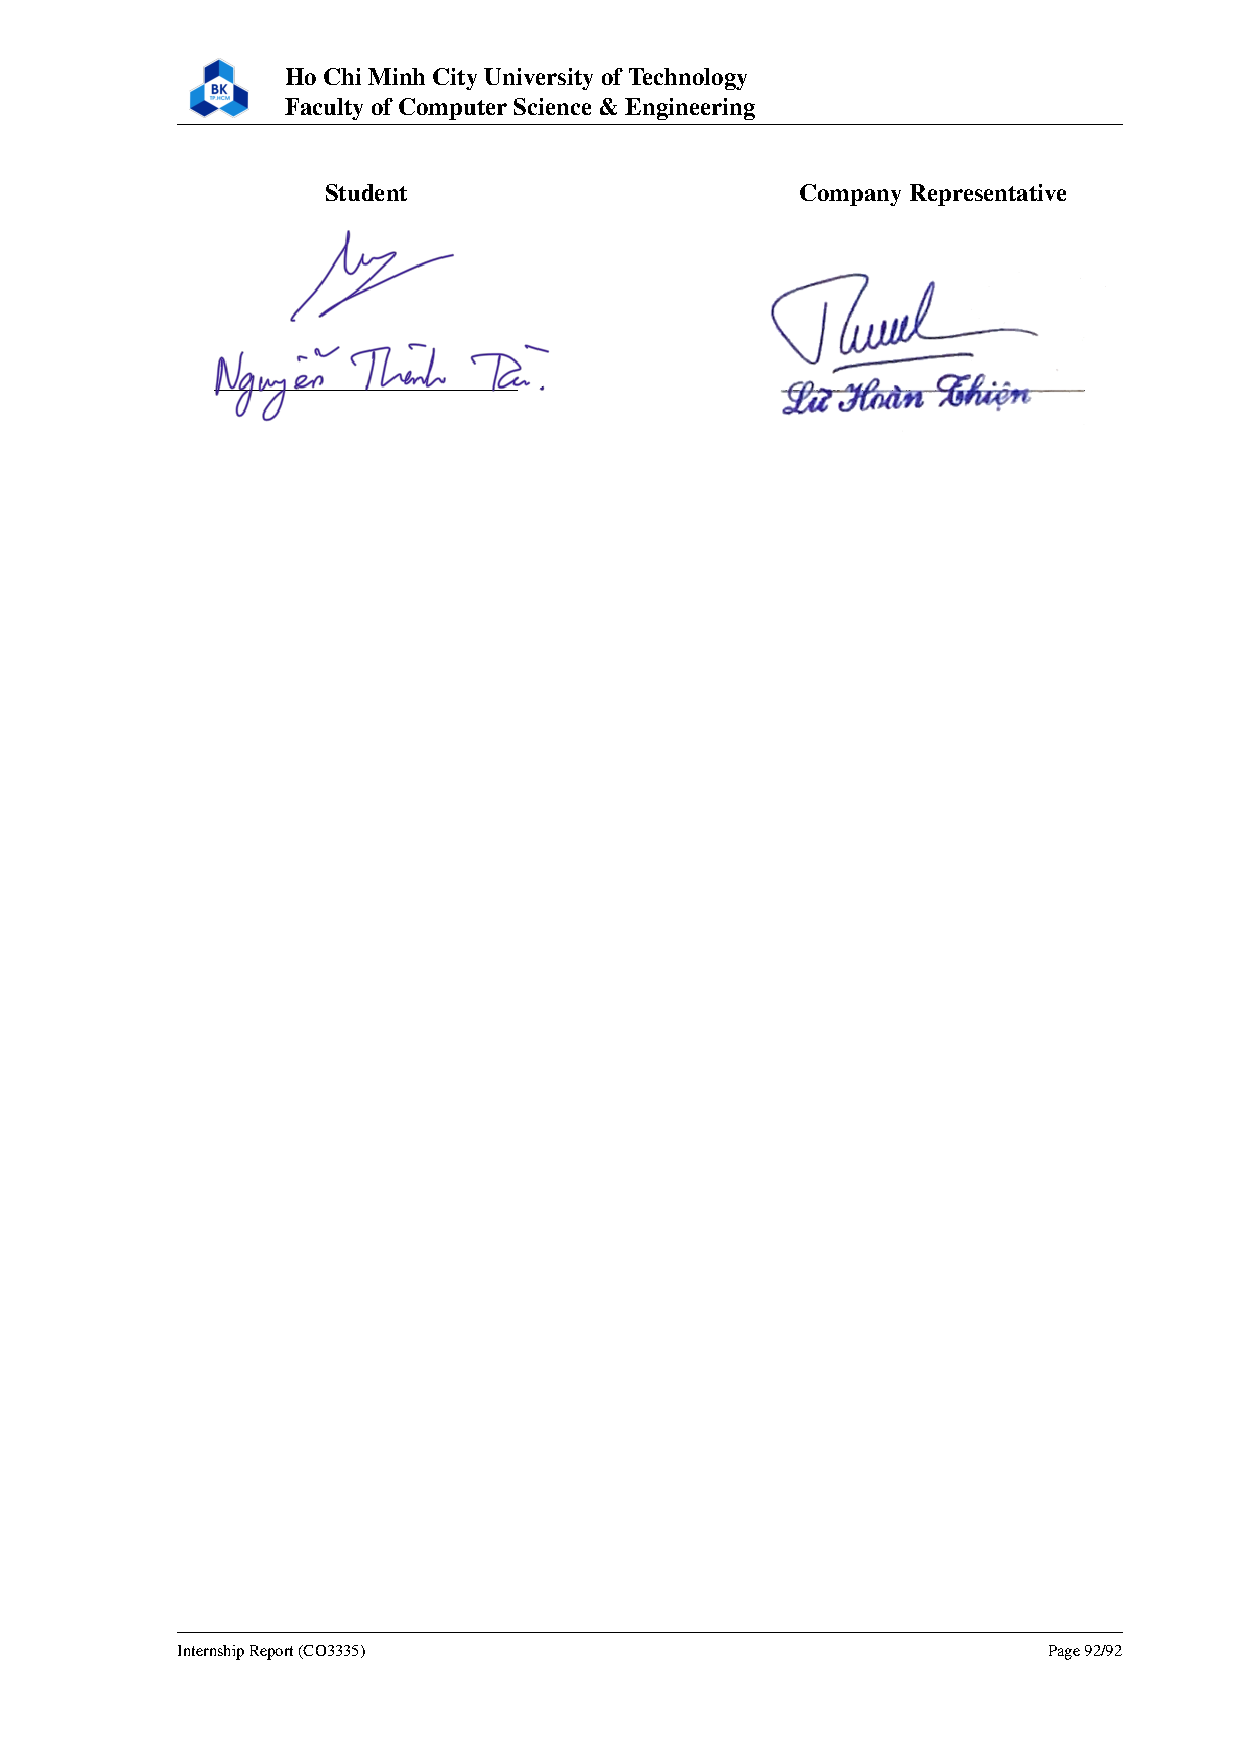
\includepdf[pages=-,pagecommand={\thispagestyle{empty}}]{form/TongKet.pdf}
}{
\newpage
\vspace{1cm}

\begin{center}
\begin{minipage}[t]{0.4\textwidth}
    \centering
    \textbf{Sinh viên}\\[0.2cm]
    % (Kí và ghi rõ họ tên)

    \vspace{2.5cm}

    \rule{0.8\linewidth}{0.4pt}
\end{minipage}
\hfill
\begin{minipage}[t]{0.4\textwidth}
    \centering
    \textbf{Người đại diện doanh nghiệp}\\[0.2cm]
    % (Kí và ghi rõ họ tên)

    \vspace{2.5cm}

    \rule{0.8\linewidth}{0.4pt}
\end{minipage}
\end{center}
}
\end{document}
